\documentclass[
      12pt,
        ]{article}






% --- type and typeface? -----------------------

% input
\usepackage[utf8]{inputenc}

% typography
\usepackage{microtype}


\usepackage[T1]{fontenc}


% text block
\usepackage{setspace}
\usepackage[              left = 1in,top = 1in,right = 1in,bottom = 1in             ]{geometry}

\usepackage{enumitem}
  \setlist{noitemsep}



% decimal numbering for appendix figs and tabs


% Deletes section counters
% \setcounter{secnumdepth}{0}



  \usepackage{color}
  \usepackage{fancyvrb}
  \newcommand{\VerbBar}{|}
  \newcommand{\VERB}{\Verb[commandchars=\\\{\}]}
  \DefineVerbatimEnvironment{Highlighting}{Verbatim}{commandchars=\\\{\}}
  % Add ',fontsize=\small' for more characters per line
  \usepackage{framed}
  \definecolor{shadecolor}{RGB}{248,248,248}
  \newenvironment{Shaded}{\begin{snugshade}}{\end{snugshade}}
  \newcommand{\AlertTok}[1]{\textcolor[rgb]{0.94,0.16,0.16}{#1}}
  \newcommand{\AnnotationTok}[1]{\textcolor[rgb]{0.56,0.35,0.01}{\textbf{\textit{#1}}}}
  \newcommand{\AttributeTok}[1]{\textcolor[rgb]{0.77,0.63,0.00}{#1}}
  \newcommand{\BaseNTok}[1]{\textcolor[rgb]{0.00,0.00,0.81}{#1}}
  \newcommand{\BuiltInTok}[1]{#1}
  \newcommand{\CharTok}[1]{\textcolor[rgb]{0.31,0.60,0.02}{#1}}
  \newcommand{\CommentTok}[1]{\textcolor[rgb]{0.56,0.35,0.01}{\textit{#1}}}
  \newcommand{\CommentVarTok}[1]{\textcolor[rgb]{0.56,0.35,0.01}{\textbf{\textit{#1}}}}
  \newcommand{\ConstantTok}[1]{\textcolor[rgb]{0.00,0.00,0.00}{#1}}
  \newcommand{\ControlFlowTok}[1]{\textcolor[rgb]{0.13,0.29,0.53}{\textbf{#1}}}
  \newcommand{\DataTypeTok}[1]{\textcolor[rgb]{0.13,0.29,0.53}{#1}}
  \newcommand{\DecValTok}[1]{\textcolor[rgb]{0.00,0.00,0.81}{#1}}
  \newcommand{\DocumentationTok}[1]{\textcolor[rgb]{0.56,0.35,0.01}{\textbf{\textit{#1}}}}
  \newcommand{\ErrorTok}[1]{\textcolor[rgb]{0.64,0.00,0.00}{\textbf{#1}}}
  \newcommand{\ExtensionTok}[1]{#1}
  \newcommand{\FloatTok}[1]{\textcolor[rgb]{0.00,0.00,0.81}{#1}}
  \newcommand{\FunctionTok}[1]{\textcolor[rgb]{0.00,0.00,0.00}{#1}}
  \newcommand{\ImportTok}[1]{#1}
  \newcommand{\InformationTok}[1]{\textcolor[rgb]{0.56,0.35,0.01}{\textbf{\textit{#1}}}}
  \newcommand{\KeywordTok}[1]{\textcolor[rgb]{0.13,0.29,0.53}{\textbf{#1}}}
  \newcommand{\NormalTok}[1]{#1}
  \newcommand{\OperatorTok}[1]{\textcolor[rgb]{0.81,0.36,0.00}{\textbf{#1}}}
  \newcommand{\OtherTok}[1]{\textcolor[rgb]{0.56,0.35,0.01}{#1}}
  \newcommand{\PreprocessorTok}[1]{\textcolor[rgb]{0.56,0.35,0.01}{\textit{#1}}}
  \newcommand{\RegionMarkerTok}[1]{#1}
  \newcommand{\SpecialCharTok}[1]{\textcolor[rgb]{0.00,0.00,0.00}{#1}}
  \newcommand{\SpecialStringTok}[1]{\textcolor[rgb]{0.31,0.60,0.02}{#1}}
  \newcommand{\StringTok}[1]{\textcolor[rgb]{0.31,0.60,0.02}{#1}}
  \newcommand{\VariableTok}[1]{\textcolor[rgb]{0.00,0.00,0.00}{#1}}
  \newcommand{\VerbatimStringTok}[1]{\textcolor[rgb]{0.31,0.60,0.02}{#1}}
  \newcommand{\WarningTok}[1]{\textcolor[rgb]{0.56,0.35,0.01}{\textbf{\textit{#1}}}}




  \usepackage{longtable, booktabs}

  \usepackage{graphicx,grffile}
  % Scale images; don't overflow page margins by default.
  % Still possible explicate \includegraphics[width, height, ...]{}
  \makeatletter
    \def\maxwidth{\ifdim\Gin@nat@width>\linewidth\linewidth\else\Gin@nat@width\fi}
    \def\maxheight{\ifdim\Gin@nat@height>\textheight\textheight\else\Gin@nat@height\fi}
  \makeatother 
  \setkeys{Gin}{width=\maxwidth,height=\maxheight,keepaspectratio}








  \usepackage{natbib}
  \bibliographystyle{apa}
  % protect underscores in most circumstances
  \usepackage[strings]{underscore} 


% 

% \newtheorem{hypothesis}{Hypothesis}

\makeatletter
  \@ifpackageloaded{hyperref}{}{%
    \ifxetex
      % page size defined by xetex
      % unicode breaks when used with xetex
      \PassOptionsToPackage{hyphens}{url}\usepackage[setpagesize = false, 
                                                     unicode = false, 
                                                     xetex]{hyperref}
    \else
      \PassOptionsToPackage{hyphens}{url}\usepackage[unicode = true]{hyperref}
    \fi
  }

  \@ifpackageloaded{color}{
    \PassOptionsToPackage{usenames,dvipsnames}{color}
  }{
    \usepackage[usenames,dvipsnames]{color}
  }
\makeatother

\hypersetup{breaklinks = true,
            bookmarks = true,
            pdfauthor = {},
             pdfkeywords  =  {},  
            pdftitle = {},
            colorlinks = true,
            citecolor = black,
            urlcolor = blue,
            linkcolor = magenta,
            pdfborder = {0 0 0}}

% \urlstyle{same}  % don't use monospace font for urls


% set default figure placement to htbp
\makeatletter
  \def\fps@figure{hbtp}
\makeatother

  \usepackage{booktabs}
  \usepackage{longtable}
  \usepackage{array}
  \usepackage{multirow}
  \usepackage{wrapfig}
  \usepackage{float}
  \usepackage{colortbl}
  \usepackage{pdflscape}
  \usepackage{tabu}
  \usepackage{threeparttable}
  \usepackage{threeparttablex}
  \usepackage[normalem]{ulem}
  \usepackage{makecell}
  \usepackage{xcolor}

% optional footnotes as endnotes


% ----- Pandoc wants this tightlist command ----------
\providecommand{\tightlist}{
  \setlength{\itemsep}{0pt}
  \setlength{\parskip}{0pt}
}





% --- title & section styles -----------------------


% title, author, date

  \author{}

% auto-format date?
  \date{\today}


% abstract
\usepackage{abstract}
  \renewcommand{\abstractname}{}    % clear the title
  \renewcommand{\absnamepos}{empty} % originally center

  \newcommand*{\authorfont}{\sffamily\selectfont}


% section titles
\usepackage[small, bf, sc]{titlesec}
  % \titleformat*{\subsection}{\itshape}
  \titleformat*{\subsubsection}{\itshape} 
  \titleformat*{\paragraph}{\itshape} 
  \titleformat*{\subparagraph}{\itshape}




% \usepackage{floatrow}
% \floatsetup[figure]{capposition=top}
% \floatsetup[table]{capposition=top}
\usepackage{multirow}
\usepackage{rotating} 
\usepackage{caption}




\begin{document}
 

% --- PAGE: title and abstract -----------------------


% \pagenumbering{gobble}




% --- PAGE: contents -----------------------




% --- PAGE: body -----------------------



\noindent 
    \hypertarget{pre-analysis}{%
\section{Pre-analysis}\label{pre-analysis}}

\hypertarget{simulated-data}{%
\subsection{Simulated Data}\label{simulated-data}}

To illustrate my planned analysis, I simulate data for each variable described above.

\textbf{Dependent variable:} \emph{Coalition success} is drawn from a descrete distribution \{-1, -.5, 0, .5, 1\}.

\textbf{Explanatory variables:} \emph{Coalition size} (a count) is drawn from a Poisson distribution. \emph{Business colation} is binomial. In reality, business coalitions are more common than non-business coalitions, but here I estimate a balanced sample. I set rule pages constant at 85 and draw \emph{comment lengths} from a Poisson distribution. While in reality, less than one percent of coalitions lobbying in rulemaking opt for a mass-comment campaign, I aim to gather a balanced sample, so half of the simulated data are assumed to have no mass comment campaign (\emph{comments} = 1, \emph{log(comments)} = 0) and the other half have a number of \emph{comments} drawn from a Zero-Truncated Poisson distribution, which is then transformed to a log scale.

\begin{Shaded}
\begin{Highlighting}[]
\NormalTok{coalition_success <-}\StringTok{ }\KeywordTok{sample}\NormalTok{(}\DataTypeTok{x =} \KeywordTok{c}\NormalTok{(}\OperatorTok{-}\DecValTok{1}\NormalTok{, }\FloatTok{-.5}\NormalTok{, }\DecValTok{0}\NormalTok{, }\FloatTok{.5}\NormalTok{, }\DecValTok{1}\NormalTok{), }\DecValTok{1000}\NormalTok{, }\DataTypeTok{prob =} \KeywordTok{c}\NormalTok{(}\FloatTok{0.1}\NormalTok{, }\FloatTok{0.3}\NormalTok{, }\FloatTok{.1}\NormalTok{, }\FloatTok{0.4}\NormalTok{, }\FloatTok{0.1}\NormalTok{), }\DataTypeTok{replace =}\NormalTok{ T)}

\NormalTok{d =}\StringTok{ }\KeywordTok{tibble}\NormalTok{(}\DataTypeTok{rule_id =} \KeywordTok{c}\NormalTok{(}\DecValTok{1}\OperatorTok{:}\DecValTok{1000}\NormalTok{, }\KeywordTok{rep}\NormalTok{(}\DecValTok{1001}\OperatorTok{:}\DecValTok{1500}\NormalTok{, }\DecValTok{2}\NormalTok{)),}
           \DataTypeTok{coalition_id =} \KeywordTok{sample}\NormalTok{(}\DecValTok{1}\OperatorTok{:}\DecValTok{2000}\NormalTok{),}
           \DataTypeTok{coalitions  =} \KeywordTok{c}\NormalTok{(}\KeywordTok{rep}\NormalTok{(}\DecValTok{1}\NormalTok{, }\DecValTok{1000}\NormalTok{), }\KeywordTok{rep}\NormalTok{(}\DecValTok{2}\NormalTok{, }\DecValTok{1000}\NormalTok{)),}
           \DataTypeTok{coalition_unopposed =} \KeywordTok{c}\NormalTok{(}\KeywordTok{rep}\NormalTok{(}\DecValTok{0}\NormalTok{, }\DecValTok{1000}\NormalTok{), }\KeywordTok{rep}\NormalTok{(}\DecValTok{1}\NormalTok{, }\DecValTok{1000}\NormalTok{)),}
           \DataTypeTok{coalition_success =} \KeywordTok{c}\NormalTok{(coalition_success, }\KeywordTok{sort}\NormalTok{(coalition_success)), }
           \DataTypeTok{coalition_size =} \KeywordTok{rtnorm}\NormalTok{(}\DecValTok{1000}\NormalTok{, }\DataTypeTok{mean =} \DecValTok{5}\NormalTok{, }\DataTypeTok{sd=} \DecValTok{10}\NormalTok{, }\DataTypeTok{lower =} \DecValTok{1}\NormalTok{) }\OperatorTok\StringTok{ }\KeywordTok{rep}\NormalTok{(}\DecValTok{2}\NormalTok{) }\OperatorTok\StringTok{ }\KeywordTok{round}\NormalTok{(), }
           \DataTypeTok{coalition_business =} \KeywordTok{sample}\NormalTok{(}\DataTypeTok{x =} \KeywordTok{c}\NormalTok{(}\DecValTok{0}\NormalTok{,}\DecValTok{1}\NormalTok{), }\DecValTok{2000}\NormalTok{, }\DataTypeTok{replace =}\NormalTok{ T, }\DataTypeTok{prob =} \KeywordTok{c}\NormalTok{(}\FloatTok{0.3}\NormalTok{, }\FloatTok{.7}\NormalTok{)), }
           \DataTypeTok{comment_length =} \KeywordTok{round}\NormalTok{(}\KeywordTok{rpois}\NormalTok{(}\DecValTok{2000}\NormalTok{, }\DecValTok{10}\NormalTok{)}\OperatorTok{/}\DecValTok{85} \OperatorTok{*}\DecValTok{100}\NormalTok{, }\DecValTok{1}\NormalTok{), }
           \DataTypeTok{comments=} \KeywordTok{c}\NormalTok{(}\KeywordTok{rtnorm}\NormalTok{(}\DecValTok{1000}\NormalTok{, }\DataTypeTok{mean =} \DecValTok{10000}\NormalTok{, }\DataTypeTok{sd =} \DecValTok{100000}\NormalTok{, }\DataTypeTok{lower =} \DecValTok{100}\NormalTok{), }\KeywordTok{rep}\NormalTok{(}\DecValTok{1}\NormalTok{, }\DecValTok{1000}\NormalTok{)) }\OperatorTok\StringTok{ }\KeywordTok{sample}\NormalTok{() }\OperatorTok\StringTok{ }\KeywordTok{round}\NormalTok{() , }
           \DataTypeTok{cong_support =} \KeywordTok{c}\NormalTok{(}\KeywordTok{rtnorm}\NormalTok{(}\DecValTok{1000}\NormalTok{, }\DataTypeTok{mean =} \DecValTok{1}\NormalTok{, }\DataTypeTok{sd =} \DecValTok{5}\NormalTok{, }\DataTypeTok{lower =} \DecValTok{0}\NormalTok{), }\KeywordTok{rep}\NormalTok{(}\DecValTok{0}\NormalTok{, }\DecValTok{1000}\NormalTok{)) }\OperatorTok\StringTok{ }\KeywordTok{sample}\NormalTok{() }\OperatorTok\StringTok{ }\KeywordTok{round}\NormalTok{() )}

\NormalTok{d }\OperatorTok\StringTok{ }\KeywordTok{sample_n}\NormalTok{(}\DecValTok{10}\NormalTok{) }\OperatorTok\StringTok{ }\NormalTok{dplyr}\OperatorTok{::}\KeywordTok{select}\NormalTok{(rule_id, coalition_id, }\KeywordTok{everything}\NormalTok{()) }\OperatorTok\StringTok{ }\NormalTok{knitr}\OperatorTok{::}\KeywordTok{kable}\NormalTok{(}\DataTypeTok{caption =} \StringTok{"Simulated data"}\NormalTok{) }\OperatorTok\StringTok{ }\KeywordTok{kable_styling}\NormalTok{(}\DataTypeTok{font_size =} \DecValTok{5}\NormalTok{)}
\end{Highlighting}
\end{Shaded}

\begin{table}[t]

\caption{\label{tab:unnamed-chunk-1}Simulated data}
\centering
\fontsize{5}{7}\selectfont
\begin{tabular}{r|r|r|r|r|r|r|r|r|r}
\hline
rule\_id & coalition\_id & coalitions & coalition\_unopposed & coalition\_success & coalition\_size & coalition\_business & comment\_length & comments & cong\_support\\
\hline
527 & 561 & 1 & 0 & 0.5 & 17 & 0 & 20.0 & 60885 & 0\\
\hline
554 & 1378 & 1 & 0 & 0.5 & 3 & 1 & 16.5 & 59688 & 9\\
\hline
1187 & 1287 & 2 & 1 & -0.5 & 24 & 0 & 10.6 & 111855 & 0\\
\hline
1328 & 1066 & 2 & 1 & -0.5 & 9 & 1 & 15.3 & 1 & 0\\
\hline
1289 & 750 & 2 & 1 & 0.5 & 14 & 1 & 16.5 & 189593 & 4\\
\hline
170 & 635 & 1 & 0 & 0.5 & 15 & 1 & 9.4 & 24996 & 7\\
\hline
107 & 786 & 1 & 0 & 0.5 & 24 & 1 & 14.1 & 25592 & 3\\
\hline
88 & 1376 & 1 & 0 & -0.5 & 9 & 1 & 9.4 & 93001 & 5\\
\hline
740 & 329 & 1 & 0 & 0.5 & 8 & 0 & 15.3 & 1 & 2\\
\hline
743 & 1119 & 1 & 0 & 0.0 & 17 & 0 & 12.9 & 1 & 2\\
\hline
\end{tabular}
\end{table}

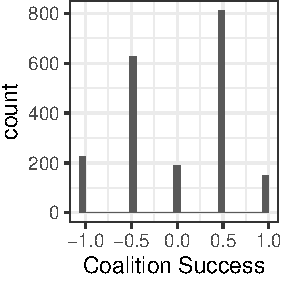
\includegraphics{Figs/hist_coalitions-1.pdf} 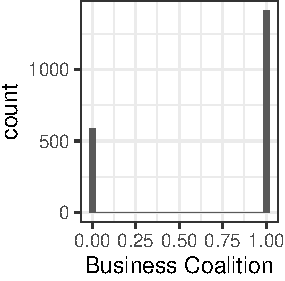
\includegraphics{Figs/hist_coalitions-2.pdf} 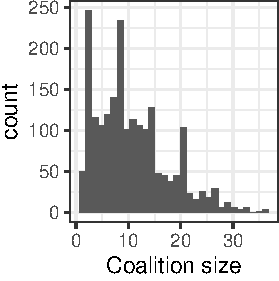
\includegraphics{Figs/hist_coalitions-3.pdf}

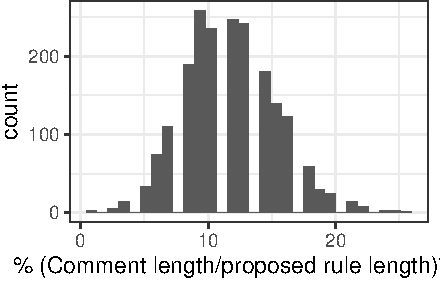
\includegraphics{Figs/hist_comments-1.pdf} 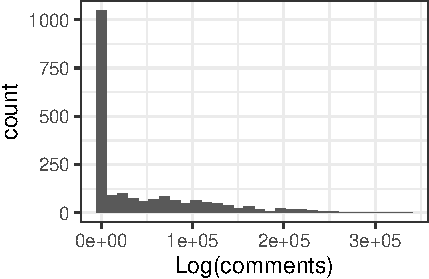
\includegraphics{Figs/hist_comments-2.pdf}

\hypertarget{simulated-results}{%
\subsection{Simulated Results}\label{simulated-results}}

Unsurprisingly this model yields no significant results. With lobbying success as the dependent variable, the coefficient on the main variable of interest would be interpreted as a one-unit increase in the logged number of comments corresponds to a \(\beta_{logmasscomments}\) increase in the five-point influence scale.

\begin{Shaded}
\begin{Highlighting}[]
\NormalTok{m <-}\StringTok{ }\KeywordTok{lm}\NormalTok{(coalition_success }\OperatorTok{~}\StringTok{ }\KeywordTok{log}\NormalTok{(comments) }\OperatorTok{+}\StringTok{ }
\StringTok{          }\NormalTok{comment_length }\OperatorTok{+}\StringTok{ }
\StringTok{          }\NormalTok{coalition_business }\OperatorTok{+}\StringTok{  }
\StringTok{          }\NormalTok{coalition_size }\OperatorTok{+}\StringTok{ }
\StringTok{          }\NormalTok{coalition_unopposed, }
        \DataTypeTok{data =}\NormalTok{ d) }
\end{Highlighting}
\end{Shaded}

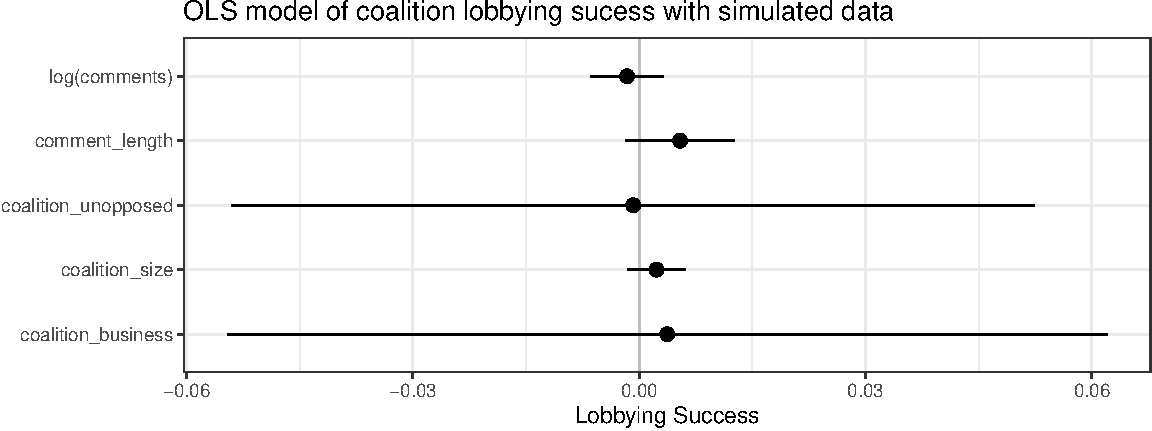
\includegraphics{Figs/model_success_plot-1.pdf}

To assess congressional support as a mediator in the influence of public pressure campaigns on rulemaking, I estimate the average conditional marginal effect (ACME, conditional on the number of comments from Members of Congress) and average direct effect (ADE) of mass comments using causal mediation analysis.

\begin{Shaded}
\begin{Highlighting}[]
\KeywordTok{library}\NormalTok{(mediation)}

\CommentTok{# model predicting mediator}
\NormalTok{model.m <-}\StringTok{ }\KeywordTok{lm}\NormalTok{(cong_support }\OperatorTok{~}\StringTok{  }\KeywordTok{log}\NormalTok{(comments) }\OperatorTok{+}\StringTok{ }\NormalTok{comment_length }\OperatorTok{+}\StringTok{ }\NormalTok{coalition_business}\OperatorTok{+}\StringTok{  }\NormalTok{coalition_size }\OperatorTok{+}\StringTok{ }\NormalTok{coalition_unopposed, }\DataTypeTok{data =}\NormalTok{ d) }

\CommentTok{# model predicting DV}
\NormalTok{model.y <-}\StringTok{ }\KeywordTok{lm}\NormalTok{(coalition_success }\OperatorTok{~}\StringTok{ }\KeywordTok{log}\NormalTok{(comments) }\OperatorTok{+}\StringTok{ }\NormalTok{cong_support }\OperatorTok{+}\StringTok{ }\NormalTok{comment_length }\OperatorTok{+}\StringTok{ }\NormalTok{coalition_business}\OperatorTok{+}\StringTok{  }\NormalTok{coalition_size }\OperatorTok{+}\StringTok{ }\NormalTok{coalition_unopposed, }\DataTypeTok{data =}\NormalTok{ d) }

\NormalTok{med.cont <-}\StringTok{ }\KeywordTok{mediate}\NormalTok{(model.m, model.y, }\DataTypeTok{sims=}\DecValTok{1000}\NormalTok{, }\DataTypeTok{treat =} \StringTok{"log(comments)"}\NormalTok{,}
\DataTypeTok{mediator =} \StringTok{"cong_support"}\NormalTok{)}

\KeywordTok{summary}\NormalTok{(med.cont)}
\end{Highlighting}
\end{Shaded}

\begin{verbatim}
## 
## Causal Mediation Analysis 
## 
## Quasi-Bayesian Confidence Intervals
## 
##                 Estimate 95% CI Lower 95% CI Upper p-value
## ACME            4.54e-06    -1.10e-04         0.00    0.91
## ADE            -1.71e-03    -6.28e-03         0.00    0.50
## Total Effect   -1.71e-03    -6.28e-03         0.00    0.50
## Prop. Mediated -4.02e-04    -1.86e-01         0.16    0.94
## 
## Sample Size Used: 2000 
## 
## 
## Simulations: 1000
\end{verbatim}
% --- PAGE: endnotes -----------------------
% --- PAGE: refs -----------------------
\newpage
\singlespacing 
          \bibliography{mendeley.bib} 
  \end{document}
